\scanpage{81}
groupes fondamentaux
\[
(54)\qquad
\diagram{\begin{tikzcd}[ampersand replacement=\&,row sep=large,column sep=large]
\&\Pi\arrow[dl,hook]\arrow[dr,hook,no head]\&\\
\Pi^D\arrow[dr,hook]\&\&\Pi^\tau\arrow[dl,hook]\\
\&\Pi^{D,\tau}\&
\end{tikzcd}}
\]
Pour exprimer commodément des générateurs remarquables de ces groupes, on introduit des chemins (indexés par \inserted{les} $a\in A$, i.e. les \uline{arêtes} du polygône)
\[
(55)\qquad \lambda_a:P_{\omega'}\longrightarrow P_\omega
\qquad
\begin{gathered}
\deleted{demi}\inserted{arc de} \text{ demi-grand cercle}\\
\text{passant par }Q_a
\end{gathered}
\]
Pour tout $s\in S$, soit
\[
\left\{
\begin{gathered}
a(s,\omega)\text{ ou }a(s)\in A\text{ tel que }(s,a)\text{ soit un repère}\\
\text{d'orientation }\omega,\text{ i.e. }
\deleted{\unsure{avec }a(\omega s,\omega)=\omega a(s,\omega)}
\inserted{s=\operatorname{or}_{\omega}(a)}
\end{gathered}
\right.
\]
\figure{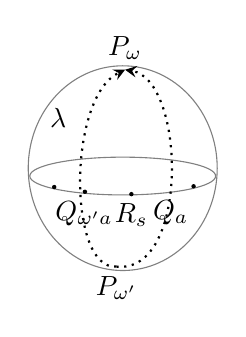
\begin{tikzpicture}[x=1cm,y=1cm,>=stealth]
\draw[gray,thin] (0,0) ellipse (1.2 and 1.3);
\draw[gray,thin] (0,-.1) ellipse (1.18 and .24);
\coordinate (N) at (.03,1.25);\coordinate (S) at (-.08,-1.25);
\draw[thick,dotted,->] (S) .. controls (-.7,-1.3) and (-.7,.9) .. (N);
\draw[thick,dotted,->] (S) .. controls (.85,-1.35) and (.8,1.12) .. (N);
\node[above] at (N) {$P_\omega$};\node[below] at (S) {$P_{\omega'}$};
\foreach \x/\y in {-.87/-.24,-.48/-.30,.11/-.33,.9/-.23}
{\fill (\x,\y) circle (.028);}
\node[below] at (-.49,-.30) {$Q_{\omega'a}$};
\node[below] at (.11,-.33) {$R_s$};
\node[below] at (.61,-.29) {$Q_a$};
\node at (-.82,.64) {$\lambda$};
\end{tikzpicture}}
on posera
\[
(56)\qquad
\begin{gathered}
\rho_s=\lambda_a\lambda_{\omega'(a)}^{-1}\\
\in\,\Pi_P=\Pi_1(\Sigma_P^*,P_\omega)
\end{gathered}
\quad
\begin{gathered}
\text{où }a=a(s,\omega),\ \omega'=\omega^{-1}\\
\text{donc }\omega'(a)=a(\omega'(s),\omega)
\end{gathered}
\]
On aura alors, pour tout $s\in S$
\[
(57)\qquad
\rho_{\omega^{n-1}s}\rho_{\omega^{n-2}s}\cdots\rho_{\omega s}\rho_s=1.
\]
Toutes ces $n$ relations sont équivalentes entre elles, si on choisit un sommet origine $s_0$ -- ce qui, avec le choix de $\omega$, fait un \uline{repère} \deleted{\unsure{de}} $r=(s_0,a(s_0,\omega))$ de $P$, d'où aussi un repère de la carte cyclotomique associée), on pose aussi
\[
(58)\qquad \rho_i=\rho_{\omega^i s_0}
\qquad
\begin{gathered}
(i\in\mathbb Z/n\mathbb Z\text{ -- les indices}\\
\text{sont notés le plus souvent}\\
0,1,\ldots,n-1
\end{gathered}
\]
de sorte que (57) prend la forme
\margin{80}
